\documentclass[12pt]{article}
\usepackage[utf8]{inputenc}
\usepackage[T1]{fontenc} % uses T1 fonts (better quality)
\usepackage{lmodern}
\usepackage[dvipsnames]{xcolor}
\usepackage[margin=2cm]{geometry}
\geometry{top=1.5cm}
\usepackage{graphicx} \graphicspath{ {./Images/} }
\usepackage{pdfpages}
\usepackage{booktabs}   % for table borders
\usepackage{amsmath,bm,amssymb}
\usepackage{mathtools}
\usepackage[makeroom]{cancel}
\usepackage{tikz} \usetikzlibrary{shapes,arrows}
\usepackage{minted} \usemintedstyle{friendly}
\usepackage{enumitem}
\makeatletter
\renewcommand{\thefigure}{8.\@arabic\c@figure}

\makeatother
\usepackage{fancyhdr}
\pagestyle{fancy}
\fancyhf{}
\lhead{ECE540}
\chead{Homework \#4}
\rhead{David Kirby}
\cfoot{\thepage}

\begin{document}
\thispagestyle{empty}

 	\begin{center}
    \line(1,0){300}\\[0.25cm]
 	\Large{\bfseries ECE540: Homework \#4}\\
 	\textsc{\large David Kirby}\\
 	\textsc{\large Due: 08 November 2020}\\
 	\line(1,0){300}\\[0.75cm]
 	\end{center}
% Define block styles
% \tikzstyle{decision} = [diamond, draw, fill=blue!20,
%     text width=4.5em, text badly centered, node distance=3cm, inner sep=0pt]
% \tikzstyle{block} = [rectangle, draw,
%     text width=20em, text centered, rounded corners, minimum height=1em]
% \tikzstyle{line} = [draw, -latex']
% \tikzstyle{cloud} = [draw, ellipse,fill=red!20, node distance=3cm,
%     minimum height=2em]
% \noindent
\section*{Chapter 8 (\(\bm{7^{th}}\) Edition)}
\subsection*{Review Questions}
\begin{enumerate}
\subsubsection*{Section 8.1}
\item R1. What are the differences between message confidentiality and message integrity? Can you have confidentiality without integrity? Can you have integrity without confidentiality? Justify your answer.
\subsubsection*{Section 8.2}
\item R3. From a service perspective, what is an important difference between a symmetric-key system and a public-key system?
\item R4. Suppose that an intruder has an encrypted message as well as the decrypted version of that message. Can the intruder mount a ciphertext-only attack, a known-plaintext attack, or a chosen- plaintext attack?
\item R5. Consider an 8-block cipher. How many possible input blocks does this cipher have? How many possible mappings are there? If we view each mapping as a key, then how many possible keys does this cipher have?
\item R7. Suppose \(n=10,000,\ a=10,023,\ b=10,004\). Use an identity of modular arithmetic to calculate in your head \( (a \cdot b)\mod{n}\).
\end{enumerate}

\subsection*{Problems}
\begin{enumerate}
	\item P1. Using the monoalphabetic cipher in Figure 8.3, encode the message “This is an easy problem.” Decode the message “rmij’u uamu xyj.”
	\setcounter{figure}{2}
		\begin{figure}[h!]
		\centering
		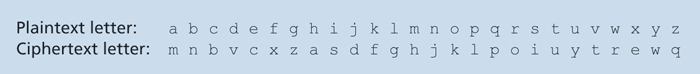
\includegraphics[width=0.85\textwidth]{./Images/Fig08-003.png}
		\caption{A monoalphabetic cipher}
		% \label{fig:I2Cdemo}
		\end{figure}
	\item P2. Show that Trudy’s known-plaintext attack, in which she knows the (ciphertext, plaintext) translation pairs for seven letters, reduces the number of possible substitutions to be checked in the example in Section 8.2.1 by approximately \(10^9\).
	\item P9. In this problem, we explore the Diffie-Hellman (DH) public-key encryption algorithm, which allows two entities to agree on a shared key. The DH algorithm makes use of a large prime number \(p\) and another large number \(g\) less than \(p\). Both \(p\) and \(g\) are made public (so that an attacker would know them). In DH, Alice and Bob each independently choose secret keys, \(S_A\) and \(S_B\), respectively. Alice then computes her public key, \(T_A\), by raising \(g\) to \(S_A\) and then taking \(\mod{p}\). Bob similarly computes his own public key \(S_B\) by raising \(g\) to \(S_B\) and then taking \(\mod{p}\). Alice and Bob then exchange their public keys over the Internet. Alice then calculates the shared secret key \(S\) by raising \(T_B\) to \(S_A\) and then taking\(\mod{p}\). Similarly, Bob calculates the shared key \(S'\) by raising \(T_A\) to \(S_B\) and then taking\(\mod{p}\).
		\begin{enumerate}
			\item Prove that, in general, Alice and Bob obtain the same symmetric key, that is, prove \(S=S'\)
			\item With \(p=11\) and \(g=2\), suppose Alice and Bob choose private keys \(S_A=5\) and \(S_B=12\), respectively. Calculate Alice’s and Bob’s public keys, \(T_A\) and \(T_B\). Show all work.
			\item Following up on part (b), now calculate \(S\) as the shared symmetric key. Show all work.
			\item Provide a timing diagram that shows how Diffie-Hellman can be attacked by a man-in-the-middle. The timing diagram should have three vertical lines, one for Alice, one for Bob, and one for the attacker Trudy.
		\end{enumerate}
	\item P12. Suppose Alice and Bob share two secret keys: an authentication key \(S_1\) and a symmetric encryption key \(S_2\). Augment Figure 8.9 so that both integrity and confidentiality are provided.
	\setcounter{figure}{8}
	\begin{figure}[h!]
	\centering
	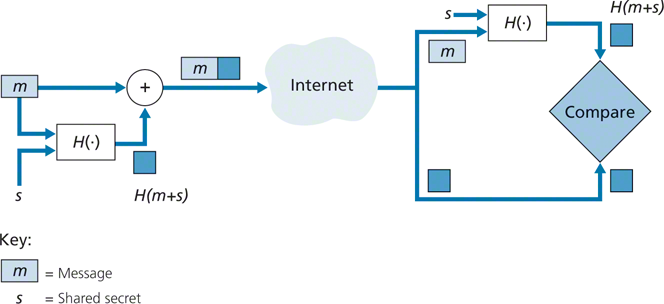
\includegraphics[width=0.85\textwidth]{./Images/Fig08-009.png}
	\caption{Message authentication code (MAC)}
	% \label{fig:I2Cdemo}
	\end{figure}
	\item P15. Consider our authentication protocol in Figure 8.18 in which Alice authenticates herself to Bob, which we saw works well (i.e., we found no flaws in it). Now suppose that while Alice is authenticating herself to Bob, Bob must authenticate himself to Alice. Give a scenario by which Trudy, pretending to be Alice, can now authenticate herself to Bob as Alice. (\textit{Hint}: Consider that the sequence of operations of the protocol, one with Trudy initiating and one with Bob initiating, can be arbitrarily interleaved. Pay particular attention to the fact that both Bob and Alice will use a nonce, and that if care is not taken, the same nonce can be used maliciously.)
	\item P19. Consider the Wireshark output below for a portion of an SSL session.
	\begin{enumerate}
		\item Is Wireshark packet 112 sent by the client or server?
		\item What is the server’s IP address and port number?
		\item Assuming no loss and no retransmissions, what will be the sequence number of the next TCP segment sent by the client?
		\item How many SSL records does Wireshark packet 112 contain?
		\item Does packet 112 contain a Master Secret or an Encrypted Master Secret or neither?
		\item Assuming that the handshake type field is 1 byte and each length field is 3 bytes, what are the values of the first and last bytes of the Master Secret (or Encrypted Master Secret)?
		\item The client encrypted handshake message takes into account how many SSL records?
		\item The server encrypted handshake message takes into account how many SSL records?
		\setcounter{figure}{-1}
		\begin{figure}[h!]
		\centering
		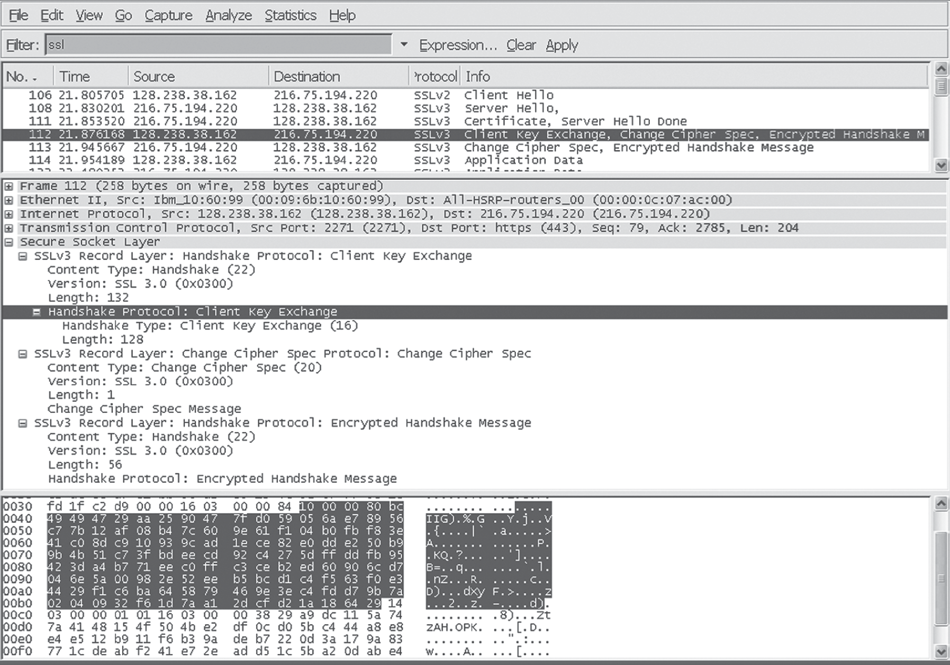
\includegraphics[width=0.85\textwidth]{./Images/UnFig08-001.png}
		\caption{(Wireshark screenshot reprinted by permission of the Wireshark Foundation.)}
		% \label{fig:I2Cdemo}
		\end{figure}
	\end{enumerate}
	\item P20. In Section 8.6.1, it is shown that without sequence numbers, Trudy (a woman-in-the middle) can wreak havoc in a TLS session by interchanging TCP segments. Can Trudy do something similar by deleting a TCP segment? What does she need to do to succeed at the deletion attack? What effect will it have?
\end{enumerate}
\end{document}